\documentclass[utf8]{gradu3}
% Jos työ on kandidaatintutkielma eikä pro gradu, käytä ylläolevan asemesta
%\documentclass[utf8,bachelor]{gradu3}
% Jos kirjoitat englanniksi, käytä ylläolevan asemesta
%\documentclass[utf8,english]{gradu3}
% tai
%\documentclass[utf8,bachelor,english]{gradu3}

\usepackage{graphicx} % kuvien mukaan ottamista varten

\usepackage{amsmath} % hyödyllinen jos tekstisi sisältää matikkaa,
                     % ei pakollinen

\usepackage{booktabs} % hyvä kauniiden taulukoiden tekemiseen

\usepackage[authordate,backend=biber,noibid]{biblatex-chicago} % biber / chicago-tyylin käyttö

\usepackage{graphicx} % kuvien lisääminen

% HUOM! Tämän tulee olla viimeinen \usepackage koko dokumentissa!
\usepackage[bookmarksopen,bookmarksnumbered,linktocpage]{hyperref}

\addbibresource{gradu_EK.bib} % Lähdetietokannan tiedostonimi

\begin{document}

\title{Vertaileva tutkimus koneoppimisen hyödyntämisestä videopelien reitinhaussa}
\translatedtitle{Comparative study of utilizing machine learning in video games' pathfinding}
\studyline{Tietotekniikka}
\tiivistelma{%
TODO: tiivistelmä suomeksi
}
\abstract{%
TODO: In english
}

\author{Emil Keränen}
\contactinformation{\texttt{emil.a.keranen@student.jyu.fi}}
% jos useita tekijöitä, anna useampi \author-komento
\supervisor{Tommi Kärkkäinen}
% jos useita ohjaajia, anna useampi \supervisor-komento
\avainsanat{koneoppiminen, videopeli, reitinhaku, syvä vahvistusoppiminen}
\keywords{machine learning, video game, pathfinding, deep reinforcement learning, Soft Actor Critic, Machine Learning Agents, Unity}

\maketitle

\bigskip

\mainmatter

\chapter{Johdanto}

- Tutkimuksen kohteena koneoppimisen tehostama reitinhaku videopeleissä
 ja sen vertaaminen heuristiseen A*-algoritmiin.

- Yleisesti reitinhaulla tarkoitetaan alku- ja loppupisteen välisen reitin selvittämistä. Useimmiten tarkoituksena
on löytää lyhin reitti väistellen samalla matkan varrella olevia esteitä.

- Reitinhakua tarvitaan videopelien lisäksi myös mm. robotiikassa. 

- Videopeleissä reitinhaku ilmenee pääasiassa tekoälyagenttien suorittamana toimintana, joten tässä tutkimuksessa keskitytään agentteihin.
Näitä agentteja kutsutaan myös ei-pelaaja-hahmoiksi (engl. non-player-character, NPC).

- Ei-pelaaja-hahmot ja itseasiassa videopelien reitinhaku vertautuvat hyvin robotiikkaan ja robottien reitinhakuun.

- Sekä robotiikassa että videopeleissä toiminta-alue voi muuttua hyvinkin paljon reaaliajassa, jolloin reitinhaun täytyy
sopeutua muutoksiin nopeasti. Käytetyt ratkaisut sen sijaan voivat vaihdella näiden kahden osa-alueen välillä: robotiikassa
tarkkuus ja turvallisuus nousevat tärkeimmiksi ominaisuuksiksi ja vastaavasti videopeleissä nopeus määrittää reitinhaun "hyvyyden".

- Reitinhaku on aina ollut vaativa ongelma videopeleissä, mutta nykyään reitinhaun ongelmallisuus voidaan
useimmissa tapauksissa sivuuttaa laatimalla heuristinen ratkaisu A*-algoritmin avulla.

- Koneoppiminen mahdollistaa aiemman kokemuksen hyödyntämisen myöhemmässä toiminnassa.
Agentteja voidaan kouluttaa harjoitteludatan avulla, jolloin ne oppivat toimimaan tuntemattomissa tilanteissa.
Koneoppimisen ansiosta reitinhaku-agentti voidaan opettaa toimimaan vaativissa ja
dynaamisissa pelialueissa, joissa muuttuvat esteet ja alueen labyrinttimäisyys
heikentävät A*-algoritmin toimintaa.

- Tutkimuksen ideana on käyttää Unity-pelimoottorille luotuja koneoppimisagentteja (engl. Unity Machine Learning Agents)
ja opettaa niitä erilaisten pelialueiden avulla. Opettamisen jälkeen agentteja testataan oikeilla
pelialueilla ja verrataan tuloksia A*-algoritmilla saatuihin tuloksiin.

- ML-agents perustuu PyTorch-kirjastoon ja mahdollistaa vahvistusoppimisen hyödyntämisen.

- Tensorboard-lisäosan avulla voidaan visualisoida palkkioiden keskiarvot ja opetuksen edistyminen opetuksen aikana.

- Pelialueiden on tarkoitus olla monimutkaisia ja dynaamisia, koska A*-algoritmi suoriutuu
yksinkertaisista reitinhakutehtävistä moitteettomasti.

\chapter{Reitinhaku videopeleissä}

Reitinhaulla tarkoitetaan yksinkertaisimmillaan reitin selvittämistä kahden pisteen välillä. Se on yksi videopelien tekoälyn ja myös robotiikan tunnetuimmista ja haastavimmista ongelmista, jota on tutkittu jo muutaman vuosikymmenen ajan \parencite{cui2011based,abd2015comprehensive}. Reitinhakua esiintyy monissa eri peligenreissä, kuten roolipeleissä ja reaaliaikaisissa strategiapeleissä, joissa ei-pelaaja-hahmoja (non-player-character, NPC) määrätään liikkumaan ennaltamäärättyyn tai pelaajan määräämään sijaintiin väistellen samalla vastaantulevia esteitä \parencite{cui2011based}.

\section{Pelialueen esitystavat}

Yleisin alueen esittämistapa on ruudukko (engl. grid), joka sisältää yksittäisiä ruutuja (engl. tile). Ruudut merkitään ennalta vapaiksi tai esteiksi. Vapaista ruuduista muodostetaan verkko, jolloin jokainen vapaa ruutu vastaa yhtä verkon solmuista. Vierekkäisiä solmuja yhdistävät linkit, joita pitkin reitinhaku tapahtuu. Solmujen vierekkäisyys voi tarkoittaa horisontaalista ja vertikaalista vierekkäisyyttä (neljä suuntaa) tai näiden lisäksi myös diagonaalista vierekkäisyyttä (kahdeksan suuntaa). \parencite{botea2013pathfinding,abd2015comprehensive}. Kuvio \ref{ruudukkokuva} havainnollistaa yksinkertaista ruudukkoaluetta, jossa liikkuminen tapahtuu neljään suuntaan.

\begin{figure}[h]
\centering
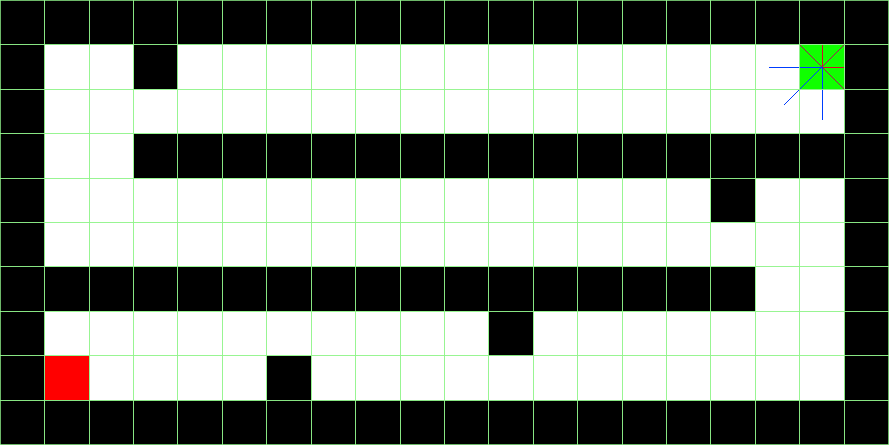
\includegraphics[width=15cm]{ruudukko_kuva.png}
\caption{Ruudukko, jossa mustat ruudut ovat esteitä ja valkoiset ruudut vapaita. Vihreä ruutu on aloitusruutu ja punainen ruutu on maaliruutu. Vihreästä ruudusta lähtevät viivat ovat mahdollisia etenemissuuntia.}
\label{ruudukkokuva}
\end{figure}

Vähemmän käytettyjä alueen esitystapoja ovat kolmiointi ja kuusikulmiointi (oikea termi kuusikulmioinnista?) \parencite{abd2015comprehensive}. Alueen kolmiointi ja siihen perustuvat TA*- ja TRA*-algoritmi ovat kuitenkin osoittautuneet moninkertaisesti nopeammiksi suurissa pelialueissa verrattuna A*-algoritmiin \parencite{demyen2006efficient}. Kuusikulmioihin perustuvat alueet ja reitinhakualgoritmit ovat myös tuottaneet lupaavia tuloksia muun muassa robotiikan tutkimuksessa \parencite{abd2015comprehensive}.

\section{Reitinhakualgoritmit}

Graafin lyhyimmän polun ongelmaa on tutkittu jo vuosikymmenten ajan. Vanhimmat ja tunnetuimmat algoritmit, Dijkstran algoritmi \parencite{dijkstra1959note} ja A*-algoritmi \parencite{hart1968formal}, esiteltiin jo 50- ja 60-luvuilla. A*-algoritmi on selvästi tunnetumpi videopelien ja robottien reitinhaussa nopeutensa ansiosta \parencite{cui2011based,abd2015comprehensive,botea2013pathfinding}. Tässä tutkimuksessa keskitytään tarkemmin A*-algoritmiin ja sen variaatioihin.

\subsection{A*-algoritmi}

A*-algoritmi on hyvin tunnettu paras-ensin -reitinhakualgoritmi (termi kuntoon?), joka hyödyntää heuristista arviointifunktiota lyhimmän reitin etsimiseen \parencite{cui2011based,duchovn2014path}.

Algoritmin toiminta tapahtuu seuraavasti: jokainen aloitussolmun vierekkäinen solmu arvioidaan kaavan f(n)=h(n)+g(n) mukaisesti, jossa n on solmu, h(n) on heuristinen etäisyys solmusta n maalisolmuun ja g(n) on todellinen etäisyys aloitussolmusta solmuun n. Näistä solmuista matalimman f(n)-arvon solmu käsitellään seuraavaksi, jolloin kyseisen solmun vierekkäisten solmujen f(n)-arvot lasketaan. Tämä prosessi jatkuu, kunnes maalisolmu saavutetaan. (oikeat matemaattiset merkinnät). Heuristiikan ollessa nolla A*-algoritmista tulee Dijkstran algoritmi.

A*-algoritmilla on kolme esitettyä ominaisuutta \parencite{hart1968formal}. A*-algoritmi löytää reitin, jos sellainen on olemassa. Reitti on optimaalinen, jos heuristiikka on luvallinen(admissible?) eli arvioitu etäisyys on lyhyempi tai yhtä suuri kuin todellinen etäisyys. Lopuksi mikään muu algoritmi samalla heuristiikalla ei käy läpi vähemmän solmuja kuin A*-algoritmi eli A* käyttää heuristiikkaa tehokkaimmalla mahdollisella tavalla. \parencite{hart1968formal,cui2011based}. Luvallisia heuristiikkoja ovat solmujen vierekkäisyydestä riippuen Euklidinen etäisyys, Manhattan-etäisyys, Chebyshev-etäisyys ja Octile-etäisyys \parencite{duchovn2014path,botea2013pathfinding}. Manhattan-etäisyyttä käytetään pääasiassa neljän suunnan ja Octile- sekä Chebyshev-etäisyyttä kahdeksan suunnan vierekkäisyyksissä \parencite{botea2013pathfinding}. Euklidista etäisyyttä voidaan käyttää tilanteessa, jossa 

\subsection{A*-algoritmin variaatiot}

A*-algoritmin heikkous on huono skaalautuvuus suurien alueiden reitinhakuun. Esimerkiksi kaksiulotteisessa ja esteettömässä 1000x1000 ruudukkoalueessa solmuja on miljoona, jolloin A*-algoritmin muistinkäyttö ja nopeus koituvat ongelmaksi. \parencite{cui2011based,duchovn2014path} Tämä ongelma esiintyy videopelien lisäksi etenkin robotiikassa, jonka seurauksena A*-algoritmi on inspiroinut tutkijoita monien eri variaatioiden kehittämiseen, kuten Theta*-, Phi*- ja HPA*-algoritmit \parencite{duchovn2014path}.

\section{Reitinhaun ongelmat}

Reitinhaun on oltava videopeleissä nopeaa ja laskennallisesti tehokasta. Lisäksi reittien on näytettävä realistiselta pelaajalle. Yhden agentin staattisen ruudukkoalueen reitinhakuongelma on ratkaistavissa nopeasti ja tehokkaasti heuristisella A*-algoritmilla, mutta nykyään videopeleissä reitinhakuongelmat ovat monimutkaisempia. Reitinhakuongelmat pitävät sisällään esimerkiksi useamman agentin samanaikaista reitinhakua ja reaaliajassa muuttuvien alueiden reitinhakua. Nykytutkimus keskittyykin pääasiassa monimutkaisiin reitinhakuongelmiin.

Useamman agentin samanaikaisessa reitinhaussa alueella on useampi kuin yksi agentti ja jokaisella niistä on oma aloitus- ja lopetuspisteensä. Jos jokaisen agentin reitinhakuun sovelletaan A*-algoritmia, on vaadittu laskennallinen teho eksponentiaalinen agenttien lukumäärän suhteen O(b potenssiin k) (tähän merkintätapa ja lähde). Laskennallisen tehon lisäksi jokaisen agentin täytyy tarvittaessa väistää toisia agentteja ja mahdollisesti muita esteitä. A*-algoritmi osoittautuu riittämättömäksi ongelman ratkaisuun.

\chapter{Koneoppiminen}

Soft Actor-Critic on Haarnojan ym. kehittämä syvä vahvistusoppimis algoritmi \parencite{haarnoja2018soft}. 

\section{Neuroverkot}

\section{Vahvistusoppiminen ja syvä vahvistusoppiminen}

\section{Soft-Actor Critic -algoritmi}

\chapter{Unity}

Unity on Unity Technologiesin kehittämä pelinkehitysalusta, joka sisältää oman renderöinti- ja fysiikkamoottorin sekä Unity Editor -nimisen graafisen käyttöliittymän \parencite{juliani2018unity}. Unityllä on mahdollista kehittää perinteisten 3D- ja 2D-pelien lisäksi myös esimerkiksi VR-pelejä tietokoneille, mobiililaitteille ja pelikonsoleille. Unitystä onkin vuosien mittaan tullut yksi tunnetuimmista pelinkehitysalustoista, jonka parissa työskentelee kuukausittain jopa 1.5 miljoonaa aktiivista käyttäjää \parencite{unityweb}.

Viime vuosina Unityä on käytetty simulointialustana tekoälytutkimuksen parissa. Unity mahdollistaa lähes mielivaltaisten tilanteiden ja ympäristöjen simuloinnin 2D ruudukkokartoista monimutkaisiin pulmanratkaisutehtäviin, joka on sen suurimpia vahvuuksia simulointialustana. Kehitystyö ja prototypointi ovat Unityllä myös erityisen nopeaa. \parencite{juliani2018unity}.

\section{Machine Learning Agents}

Machine Learning Agents on Unitylle kehitetty koneoppimispaketti, jonka avulla peliin voidaan ottaa käyttöön koneoppimisagentteja.

\chapter{Tutkimuksen empiirinen osuus}

\section{Tutkimuksen kuvaus}

\section{Tutkimusasetelma / Konfiguraatio}

\chapter{Tulokset ja johtopäätökset}

\chapter{Yhteenveto}

\printbibliography

\chapter{Liitteet}

- Kuvat tai mallinnokset pelialueesta.

- Tensorboardin kuvaajat mm. agentin palkkioiden kehityksestä.

\end{document}
